\chapter{Evaluation}
\label{chap:Evaluation}

The goal of this chapter is to evaluate different use cases for \gls{ml}-based interpolation in the context of \gls{ta} interpolation. In Chapter~\ref{chap:Machine Learning based Interpolation}, different models for \gls{ml}-based interpolation were already introduced. Afterwards, the available data and features were introduced in Chapter~\ref{chap:preparations data sets}. In this chapter, the different models are compared with different datasets and features to test the feasibility of two main use cases:

\begin{enumerate}
  \item Interpolation of \gls{ta} for a specific location
  \item Areal interpolation of \gls{ta}
\end{enumerate}

Next to these main uses cases we discuss there are other ways the different regression models can be used, primarily decided by the features used. Some regression models could for example be used to predict future \gls{ta}, i.e., extrapolation, as well; however, this is out of the scope of this work.

\subsubsection{Implementation Details}

All \gls{ml} models are implemented using Python and the scikit-learn library~\cite{scikit-learn}. Additionally, the following libraries are used:

\begin{itemize}
  \item Pandas, Numpy, Geopandas, scipy, matplotlib, shapely, contextily, pytz, sklearn, seaborn, rasterio, polars, Google Earth Engine, pykrige, pytorch, missingno
\end{itemize}

\subsubsection{Validation Methodology}
\label{sec:validation methodology}

To validate the different models, we use the following methodology:\\
We evaluate two locations based on data availability, e.g., Hamburg and Stuttgart, that also have slightly different climate characteristics, although both are located in Germany in a moderate cool climatic zone, with Hamburg located near the coast in rather Maritim climate and Stuttgart located more inland in a continental climate. Hamburg has also higher precipitation and wind compared to Stuttgart.
For both locations, we collected \gls{pws} data from Netatmo and Sensor.Community; however, Netatmo data is only available for the whole month of June 2023 for Hamburg and for a single timestep on 19. June 2023 14h for Stuttgart, while Sensor.Community data is available for the whole months of January and June 2023 for both locations.\\
For both locations for both interpolation use cases, we first compare all available models, e.g., Linear Regression, \gls{knn}, \gls{rf}, \gls{svr}, and \gls{hgb}, with all features against each other to get an understanding of the overall performance of the models and maximum achievable potential, given the assumption that more features generally improve prediction quality. The datasets are split into a training and test set. 70\% of the data is used for training and 30\% is completely withhold for testing. The training and test set are split randomly. The same split is used for all models and sensors to ensure comparability.
Afterwards, the most promising model with the lowest error is used to further evaluate specific influences such as distances between neighbours or the amount of training data and time intervals. For the further evaluation, 5-Fold Cross Validation is used to reduce the risk of overfitting~\cite{kohavi1995study}. We note here that a k of 10 would be preferred; however, due to the computational overhead we only use a k of 5 for exploration.\\
All \gls{ml} models in the initial evaluation are trained using the default parameters as defined in the scikit-learn library. The only exception is the number of estimators for the \gls{rf} Regressor and the number of iterations for the \gls{hgb} Regressor, which are both increased from 100 to 200 to improve the performance of the models as found out by previous exploration. To get the best possible performance of each model, an exhaustive grid search would be preferred for all models to fine-tune all hyperparameters; however, due to the computational overhead of running exhaustive grid searches, this is not feasible in the scope of this work.\\
For the error metrics, the following candidates are available: \gls{mse}, MAE, \gls{rmse}, \gls{r2}. \gls{mse} is the most used error metric and is more sensitive to outliers, whereas MAE punishes outliers less but is therefore also more variable. Related work commonly uses \gls{rmse} as it has the same unit as the response variable, therefore \gls{rmse} is used as the main error metric. \gls{r2} is additionally used to get an understanding of the variance of the model.

\section{Interpolation of Air Temperature for a Specific Location}

The first use-case to be evaluated is the interpolation of \gls{ta} for a specific sensor. The main idea behind this approach is to use \gls{ml} models to capture the dependency between neighbouring weather stations and sensors, so that in case a sensor is not available, the \gls{ta} can be interpolated more easily, especially over a longer period. Another use-case could be that a sensor location is not stationary, and the sensor for example moves through a city mounted on a bus or bike. In this case, the sensor could be used to capture a snapshot of the \gls{ta} at a previously unobserved location, increasing the spatial coverage of the sensor network. The evaluation for a specific location is done using the following steps:

\begin{enumerate}
  \item Create datasets for training and testing based on the datasets for June 2023 after \gls{qc} for Hamburg and Stuttgart
  \item Data pre-processing for the specific models. Only \gls{hgb} supports missing values, therefore we need to fill in missing values for all other models using an imputer. We use a simple mean imputer for this purpose, that fills missing values with the mean value for each row, i.e., each timestamp, not column. All input data is normalized using a standard scaler as some models such as \gls{knn} need normalized data, which should not have any impact on models that don't need normalization of input features such as \gls{rf} and Gradient Boosting. This pre-processing step could be further improved by using different means of imputation or using different scalers.
  \item Fit each model using the datasets and evaluate the performance using all available features for all locations to get an overview of the performance of each model. The dataset is split 70\% for training and 30\% for testing, but no k-Fold Cross Validation is used due to the computational overhead for the initial comparison across all sensor locations.
  \item Choose the most promising model and further evaluate the influence of different features, e.g., distances between neighbours, the amount of training data, and time intervals. This step only selects a subset of stations of particular interest, e.g., in the city centre or near water and adds 5-Fold Cross Validation for further trust in the results.
\end{enumerate}

\begin{figure}[ht]
  \centering
  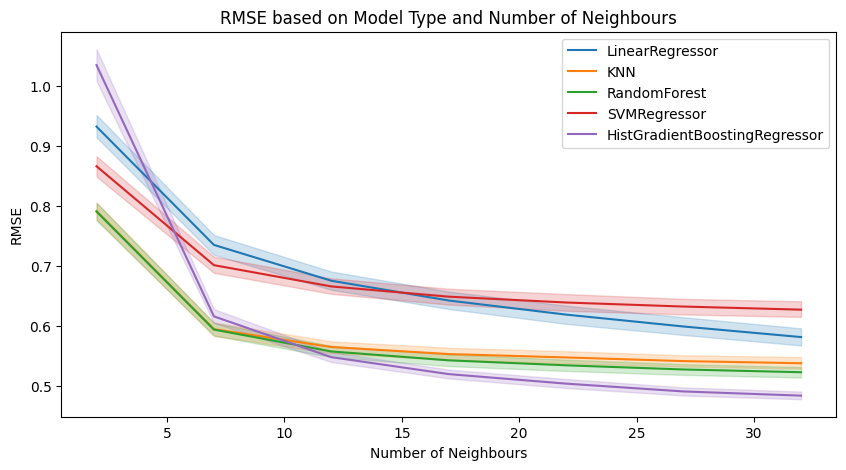
\includegraphics[width=1\textwidth]{images/rmse_by_model_type.png}
  \caption{\gls{rmse} by Model Type with the Confidence Interval of 95\%}
  \label{fig:rmse by model type}
\end{figure}

\subsection{Model Comparison}

First, we compare the overall performance of the models against each other. Figure~\ref{fig:rmse by model type} shows the \gls{rmse} of each model across both Hamburg and Stuttgart for the month of June 2023, while a more detailed overview can be found in Appendix Figure~\ref{fig:eval single station interpolation detailed} and~\ref{fig:eval single station interpolation detailed part 2}. For all models, one evaluation was done using the imputed dataset without missing values, as Linear Regression, \gls{knn}, \gls{rf} and \gls{svm} Regression cannot handle missing values. Gradient Boosting was once run with and once run without imputed data, where the imputed data performed better at 2 neighbours, possibly due to neighbours with missing values, but performed slightly worse than not imputed data for higher amounts of neighbours. \gls{svm}, \gls{knn} and \gls{rf} seem to hit a plateau when reaching a certain number of neighbours, around 15-20, whereas Linear Regression and Gradient Boosting continue to improve with a higher number of neighbours.\\
Gradient Boosting shows the lowest \gls{rmse} starting with over 10 neighbours and has the smallest confidence interval. The non-imputed data also performs slightly better, as seen in Appendix Figure~\ref{fig:eval single station interpolation detailed part 2}, therefore we will continue a more detailed evaluation with the Gradient Boosting model without imputed data. It is to note, that the individual models were mainly run with default parameters as given by sklearn library, therefore the performance of the individual models could be further improved. The exact parameter configurations can be found in Appendix~\ref{appendix: sklearn ml parameters single station}.

\subsection{Further Evaluation - Gradient Boosting}

HistGradientBoostingRegressor without imputation achieves overall the lowest \gls{rmse} starting with more than 10 neighbours and continuously improves with more neighbours; however, the improvements after 30 neighbours are small. This model is great because it has native \gls{nan} support and we can save the imputation step that can possibly introduce bias into the model. The difference to \gls{knn} and \gls{rf} is not that big with a little less than \gls{rmse} of 0.1; however, the confidence interval is also smaller compared to the other models. Due to the lowest error and performance benefits compared to other models such as \gls{rf}s and no need to use imputation, the HistGradientBoostingRegressor is used in the following section to further investigate feature importance, the influence of different time intervals and the impact of \gls{qc} on the process.\\

\begin{figure}[htp]
    \centering
    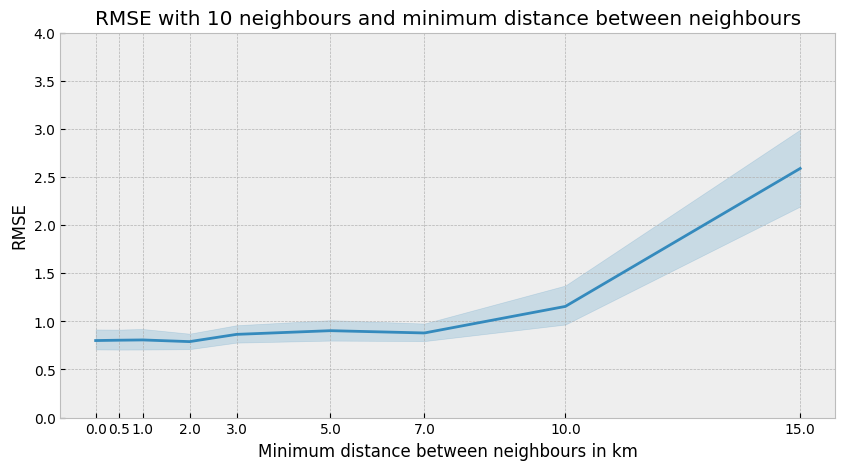
\includegraphics[width=1\textwidth]{images/rmse_10_neighbours_min_distance.png}
    \caption{\gls{rmse} for Increasing Minimum Distance with 10 Neighbours, Hamburg, Netatmo}
    \label{fig:eval hamburg minimum distance between stations}

    \centering
    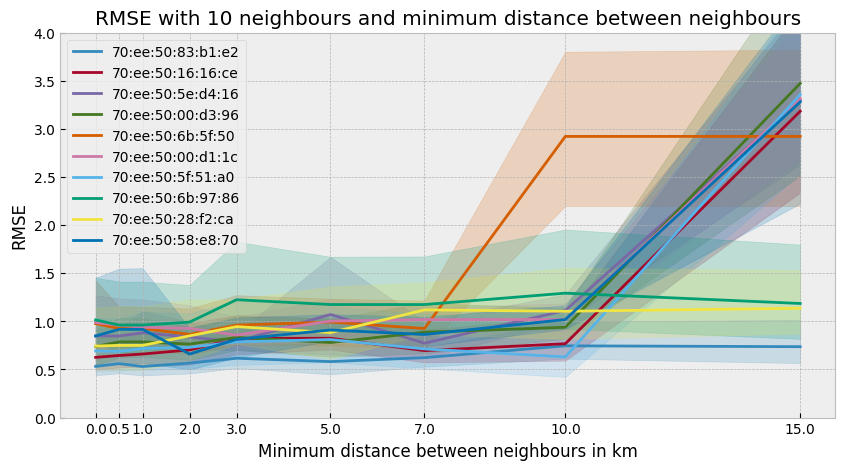
\includegraphics[width=1\textwidth]{images/rmse_10_neighbours_min_distance_by_pid.png}
    \caption{\gls{rmse} for Increasing Minimum Distance with 10 Neighbours By Station Id, Hamburg, Netatmo}
    \label{fig:eval hamburg minimum distance between stations by station id}
\end{figure}

\subsubsection{Influence of Distance between Neighbours}

% Hypotheses: closer neighbours have a higher influence on the temperature
The goal with hyperlocal temperature mapping is to get a deep insight into very local climatic conditions. If two sensors are located in the same climatic conditions, in an extreme case directly situated next to each other, both sensors should measure the same temperature. Therefore, the hypothesis is, that closer stations have a higher influence on the prediction quality, e.g., if closer stations are chosen as neighbours the prediction quality is better compared than if the same number of neighbours is chosen but further away. We investigate this hypotheses by comparing the \gls{rmse} of prediction quality for different distances between neighbours. Because there are not so many stations available for Hamburg, that for example 10 stations could be selected in a 500m radius, we look at the minimum distance instead and remove neighbours that are to close to the station.\\
The evaluation is done using 5-fold cross validation for a subset of 10 stations in Hamburg, spread across a bigger area so we can cover different distances between neighbours and different climatic conditions, e.g., distance to water, situated in the city centre etc. The list of stations can be found in Appendix~\ref{appendix stations for minimum distance between stations}. The number of neighbours was set to 10 as this number was the number at which Gradient Boosting outperformed other models. Figure~\ref{fig:eval hamburg minimum distance between stations} shows the \gls{rmse} for different minimum distances between stations in km for 10 stations from Netatmo in Hamburg with 10 neighbours. We can see that the \gls{rmse} is increasing minimally across the first few kilometres and then starts to sharply increase with greater distances over 10km. However, if we take a look at Figure~\ref{fig:eval hamburg minimum distance between stations by station id} which shows the same data but grouped by station id, we can see that there are several stations whose \gls{rmse} does not increase with greater distances.\\ % Todo: why?

\subsubsection{Feature Importance}

Next to the temperature, there are also other features that could be included in the prediction process such as the time, humidity, pressure, etc. In order to understand how much the features contribute to the overall prediction quality, we first compare the \gls{rmse} of the model with only the temperature as input feature for each neighbour, and then test with adding time, humidity, pressure, and finally all features combined. Time is only a single column of the transformed timestamp, whereas humidity and pressure are added for each neighbour. In the end the input looks as follows: [ta$_1$... ta$_n$, time, humidity$_1$... humidity$_n$, pressure$_1$... pressure$_n$]\\
Figure~\ref{fig:eval feature importance 10 stations single location} shows the \gls{rmse} for different features for 10 stations in Hamburg with 30 neighbours. We can clearly see, that there is no visible difference between only temperature and all features combined, therefore in Figure~\ref{fig:eval permutation importance single station} we take a look at the permutation importance of a single station for temperature and time on a 30\% test set. The values are calculated based on the trained regressors from the 5 different folds of the cross validation; however, the test set was always the same and not the same used during the cross-validation, due to technical limitations in the sklearn library. However, the results indicates that only a very small number of stations, in this case the neighbours 4 and 13, have a high influence on the prediction quality. All other stations have a very low influence on the prediction quality, with time having no visible influence at all. This is a very interesting result, as it indicates that the model only needs a handful of neighbours that have similar temperature distributions to the target station in order to make a good prediction. Other features such as time, humidity and pressure do not seem to have any influence on the prediction quality, and could therefore be ignored, saving computational resources and making the model more robust. This assumption could be further validated by looking at more stations and their permutation importance.\\ 

\begin{figure}[htp]
    \centering
    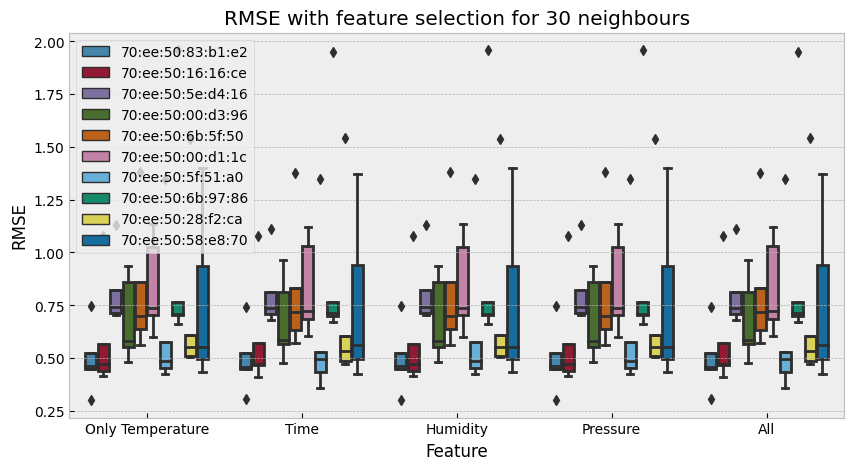
\includegraphics[width=1\textwidth]{images/rmse_30_neighbours_feature_importance_by_pid.png}
    \caption{\gls{rmse} based on Features Selected with 30 Neighbours, Hamburg, Netatmo}
    \label{fig:eval feature importance 10 stations single location}

    \centering
    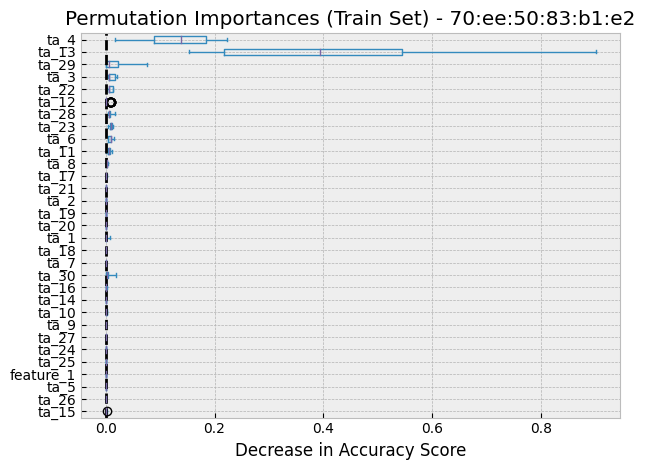
\includegraphics[width=1\textwidth]{images/rmse_30_neighbours_permutation_importance_by_pid.png}
    \caption{Permutation Importance for Single Station on 5-Fold Cross Validation, Hamburg, Netatmo}
    \label{fig:eval permutation importance single station}
\end{figure}

\subsubsection{Influence of Quality Control}

In this work, we decided to use \gls{qc} steps to exclude stations that are either faulty, setup indoors, or perhaps setup in an incorrect way (i.e., too close to a wall or the ground). However, depending on the use-case, one might want to include sensor readings that are flagged as outliers by the m5 buddy check either because the sensor density is lower or one would actually want to get a more fine-granular overview of hotspots. As a result, we compare the different \gls{qc} levels of m4 and m5, i.e., Temporal Correlation and Spatial Buddy Check, to see if the \gls{qc} levels have an influence on prediction quality of the interpolation process.\\
For this test, we use \gls{hgb} without imputed data with 30 neighbours across our 10 testing stations from Netatmo from June 2023 in Hamburg together with 5-fold Cross Validation. The result shown in Figure~\ref{fig:qc hamburg level comparison} show the smallest \gls{rmse} for the m4 \gls{qc} level, i.e., the Temporal Correlation, which could be due to the increase in data availability per station to train on. This result indicates, that maybe the m5 buddy check is too strict and maybe the \gls{qc} level m4 could be sufficient for the interpolation process.

\begin{figure}[ht]
    \centering
    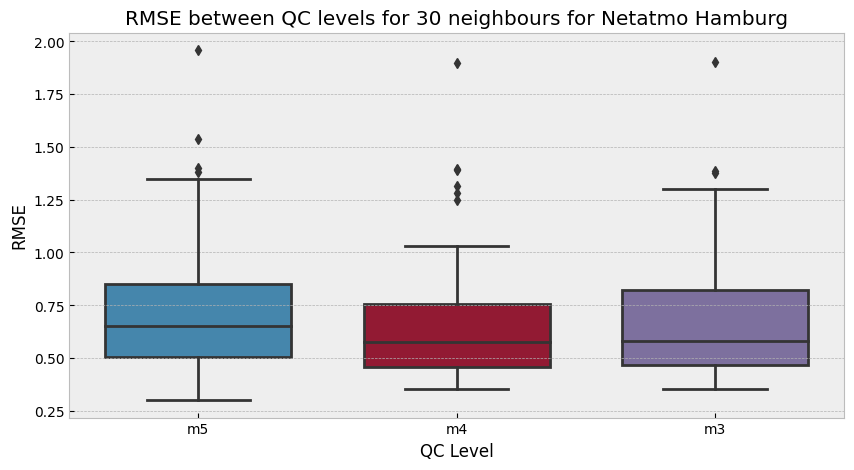
\includegraphics[width=1\textwidth]{images/qc_hamburg_level_comparison.png}
    \caption{\gls{qc} Level Comparison for Netatmo Data for Hamburg, June 2023}
    \label{fig:qc hamburg level comparison}
\end{figure}

\subsubsection{Influence of Time Intervals and Non-Stationary Sensors}

% Inplicitly included via \gls{qc} process, because many values are already missing -> check for subset with more data available how missing values influence the model

Sensor networks have the advantage, compared to remote sensing approaches, that they provide high temporal resolutions; however, at the cost of spatial coverage. In the context of \gls{ta} sensing, \gls{ta} sensors could be mounted to busses, cars, scooters, or bikes to increase the spatial coverage of the sensor network. Unfortunately, there are currently no datasets of actual moving sensors available; however, we can simulate a non-stationary sensor by removing data points of specific sensors in either a fixed interval, e.g., simulating a bus line that visits a certain location in a rather fixed interval, or randomly, simulating a bike or scooter that is used periodically.\\
We have already indirectly simulated missing data by applying \gls{qc} steps before using the station data to train the models, as seen in Section~\ref{sec:quality control}, where we lose quite some data. An interesting exploration could be to use the previous sensor with Netatmo Station Id \textit{70ee:50:83:b1:e2} and choose neighbours that have a high influence on the prediction quality, e.g., neighbour 4 and 13, and remove data points in both fixed and random intervals to simulate a moving sensor instead of a stationary sensor. We could also check what happens, if not only two but multiple neighbours are turned into simulated moving sensors.\\

\begin{figure}[ht]
    \centering
    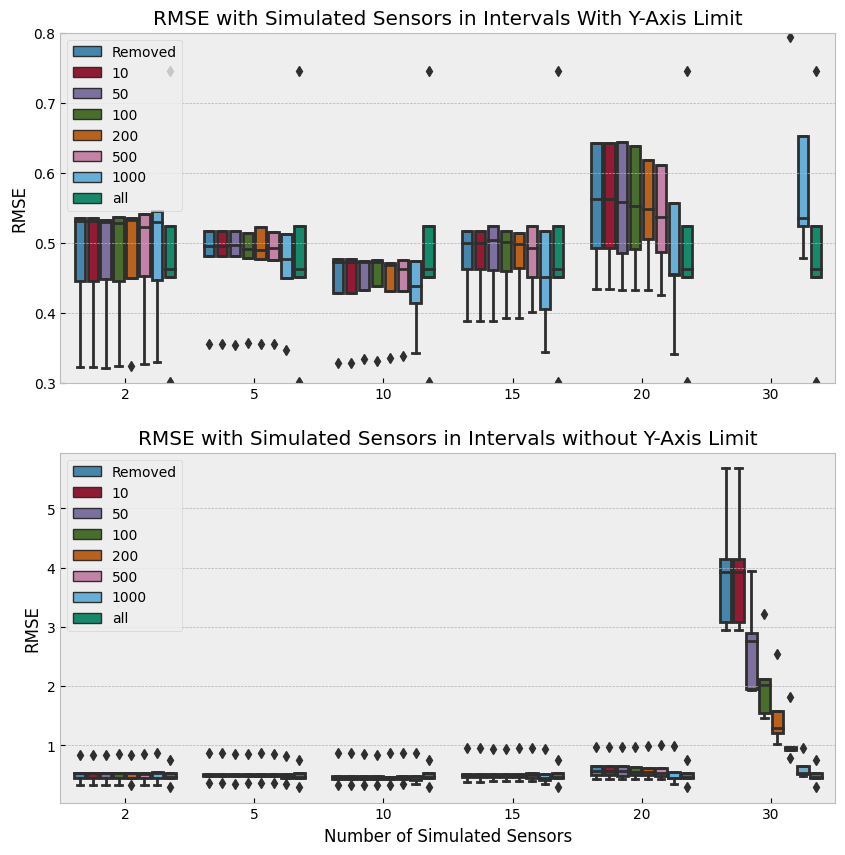
\includegraphics[width=1\textwidth]{images/eval_moving_sensors_hamburg.png}
    \caption{Comparison between amount of data sampled from simulated moving sensors for Netatmo station \textit{70ee:50:83:b1:e2} with 30 neighbours}
    \label{fig:eval moving sensors}
\end{figure}

In Figure~\ref{fig:eval moving sensors}, results are shown for the Netatmo station \textit{70ee:50:83:b1:e2} with 30 neighbours where we start off with simulating 2 sensors, i.e., \textit{70:ee:50:3f:1f:1c} and \textit{70:ee:50:96:d9:70}, which had high permutation importance, to quickly see differences between different sampling size for individual sensors. Iteratively, additional sensors were added from a list of randomly sorted neighbouring station ids, so that in each iteration the stations from the previous iteration are included. The `Removed' columns show the results with the moving sensors completely removed, while the `all' column shows what happens if all available sensor readings are used, as reference. The other numbers show the number of readings that are randomly sampled for that sensor. The number of available sensor readings per sensor is averaging around 1000-1500 readings per sensor, which was reduced from the raw data due to \gls{qc} or missing data. 5-fold cross validation was used for each combination of number of moving sensors and number of readings to sample.\\
We can see, that a low number of moving sensors, especially with high number of readings available, do not have a high influence on the \gls{rmse}, which averages between 0.5 and 0.4; however, starting with 20 moving sensors, the \gls{rmse} jumps a lot, especially with 30 moving sensors, i.e., all sensors are moving and have as little as 10 readings for the whole month of June in Hamburg. This exploration suggests, that there is not a big difference between stationary sensors and moving sensors with less frequency, as long as a certain amount of readings for that location is available and not all sensors are not available. Further research in this direction could focus on the comparison between different stations with varying number of neighbours and sample sizes. Additionally, we didn't test with fixed intervals yet, so this could also be an interesting exploration to for example simulate bus lines with sensors.

% TODO: optional
% \subsubsection{January vs June}

% TODO: optional
% \subsubsection{Neural Network Exploration}

% Areal Interpolation

\begin{figure}[htp]
    \centering
    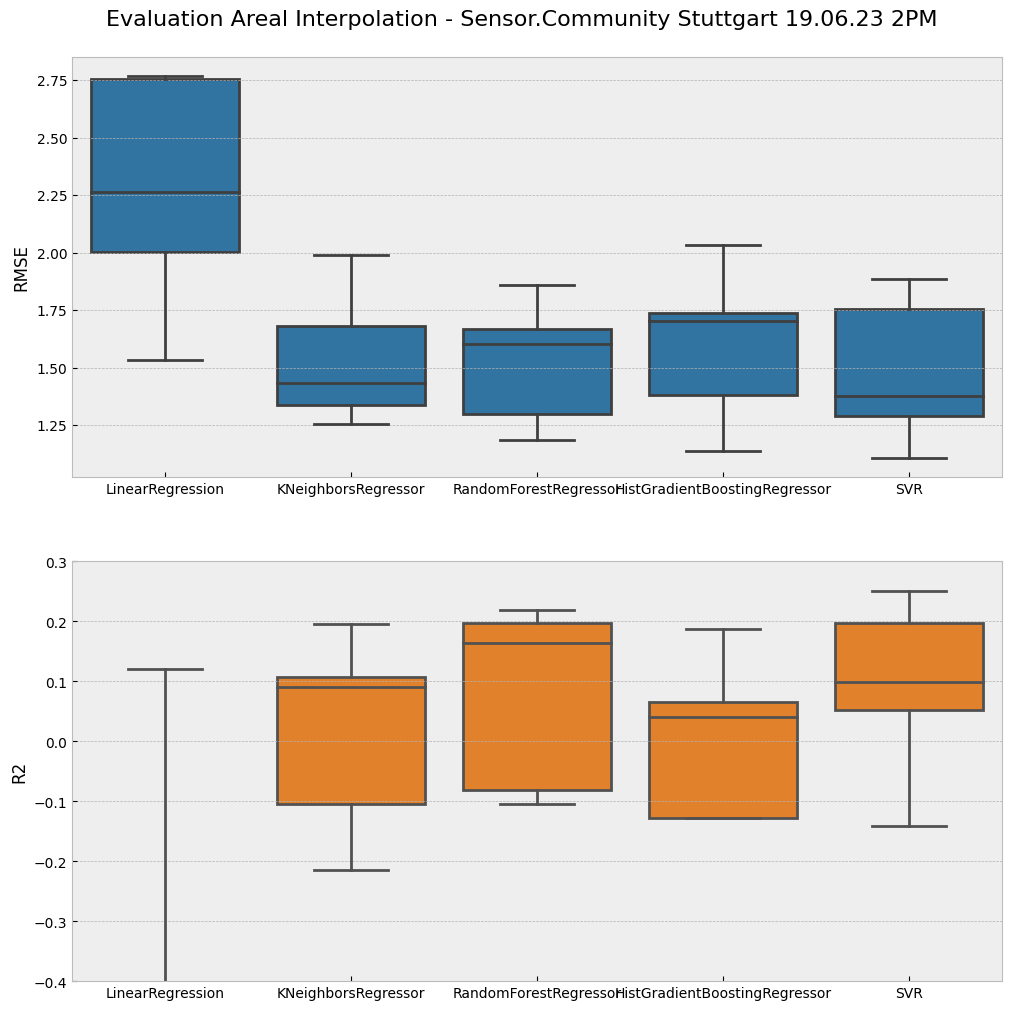
\includegraphics[width=0.9\textwidth]{images/eval areal interpolation 19.06.2023 14h.png}
    \caption{Areal Interpolation Comparison, Sensor.Community Stuttgart, 19.06.2023 2PM}
    \label{fig:eval areal interpolation 14h stuttgart}

    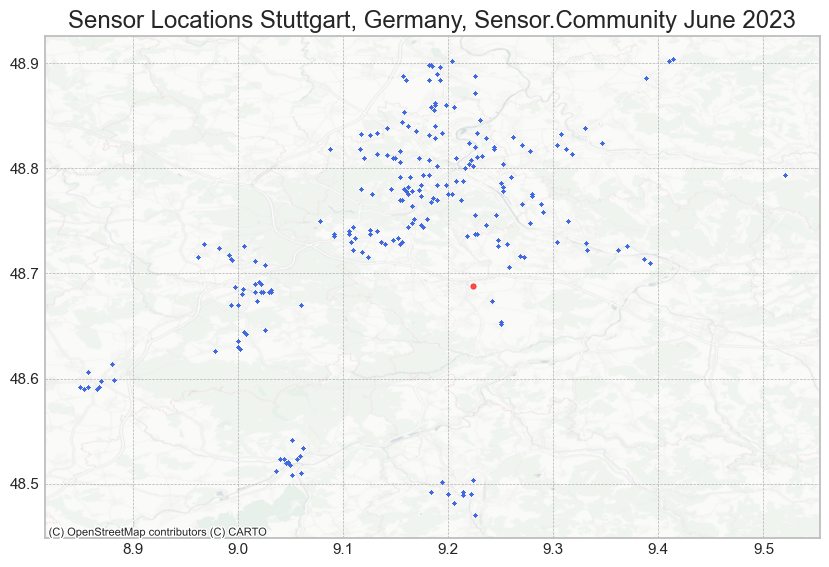
\includegraphics[width=0.9\textwidth]{images/sensor_community_locations_stuttgart_after_qc_june_23.png}
    \caption{Locations for Sensor.Community around Stuttgart, Germany, June 2023}
    \label{fig:qc sensor community stuttgart june 23}
\end{figure}

\section{Areal Interpolation of Air Temperature}

The second use-case for \gls{ml}-based interpolation of \gls{ta} is the areal interpolation, e.g., turning a set of single data points into a continuous temperature layer/grid. The problem with this approach is that in comparison to interpolating a single sensor, there are potentially many locations that have no sensor data and therefore no target variable to be trained with. The main assumption here is that locations with similar features, e.g., land coverage, soil temperature, \gls{svf}, solar radiance, etc.\ have similar \gls{ta}. This assumption is one of the motivating factors behind \gls{lcz} research. The main challenge here is to find the right features that capture the dependency between the different locations and choose how to model spatial information.\\
In the following section, areal interpolation of \gls{ta} is explored by comparing the \gls{rmse} between different models, previously discussed in Chapter~\ref{chap:Machine Learning based Interpolation}. We primarily focus on the area of Stuttgart, as Sensor.Community data for this area was much easier to acquire, as seen in Figure~\ref{fig:qc sensor community stuttgart june 23}. We focus again on the month of June 2023, as it contained a lot of periods of prolonged hot weather, as seen in the Appendix Figure~\ref{fig:dwd stuttgart june 23 mean min max}, and we are interested in mapping \gls{ta} especially during hot periods. Similar to Kriging, in our areal interpolation exploration, we focus on the interpolation of \gls{ta} for a single timestamp. Our approach could be extended in the future, to also include a temporal aspect as well; however, this is out of the scope of this work. Based on the \gls{dwd} reference station, we chose the 19.06.2023 as our reference data to try out several types of areal interpolation. To get a good understanding, what kind of \gls{ta} to expect that day, we also took a look at the 2m and 5cm \gls{ta} at the \gls{dwd} station on the 19.06.2023, as seen in Appendix Figure~\ref{fig:dwd stuttgart june 23 10 min 2m 5cm}. Interest to note here, is that the 5cm \gls{ta} fluctuates way more than the \gls{ta} at 2m, indicating that height information of a sensor place an important role, especially in areal interpolation where you cannot only rely on the relationship between neighbouring temperature curves but need to capture placement information as well.\\

\subsection{Model Comparison}

To compare the different models, we first need to define at which time we want to test our model, as we can only interpolate a single timestamp at a time. We chose the hottest temperature for the day at 2PM as well as the coldest point that day at 5AM. We start of with only Sensor.Community data and the following features:

\begin{itemize}
  \item Longitude, Latitude
  \item Humidity (where available)
  \item Pressure (where available)
  \item Indexes (500m) ->  \gls{ndvi}, EVI
  \item DEM
  \item Temperature and Distances to the closest 30 neighbours (similar to RFSP)
\end{itemize}

Each model, i.e., Linear Regression, \gls{knn}, \gls{rf}, \gls{hgb}, \gls{svm}, was run with default sklearn parameters. We used 10-fold cross validation with a StandardScaler to evaluate the model performances. The results can be found in Figure~\ref{fig:eval areal interpolation 14h stuttgart}. We can see a \gls{rmse} between 1.7 and 1.3 for \gls{knn}, \gls{rf}, \gls{hgb}, \gls{svm}, while Linear Regression clearly falls behind with over 2. The \gls{r2} score of all models is rather low with 0.2 maximum and in some cases even negative values, showing high variability during especially hot weather.\\

\begin{figure}[htp]
    \centering
    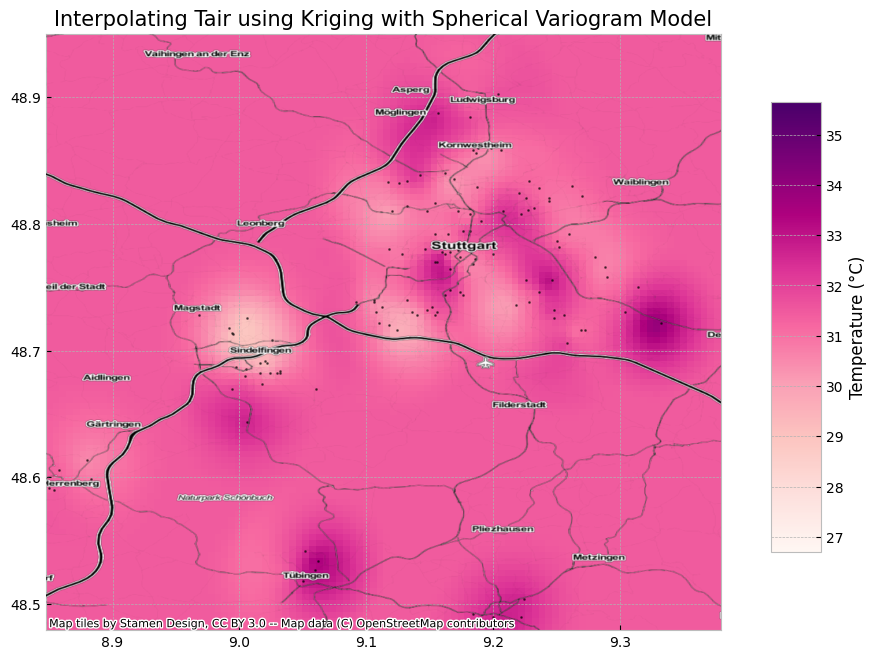
\includegraphics[width=0.9\textwidth]{images/eval areal interpolation ok stuttgart 14h.png}
    \caption{Ordinary Kriging Spherical Variogram, Sensor.Community Stuttgart, 19.06.2023 2PM}
    \label{fig:eval areal interpolation ok 14h stuttgart}

    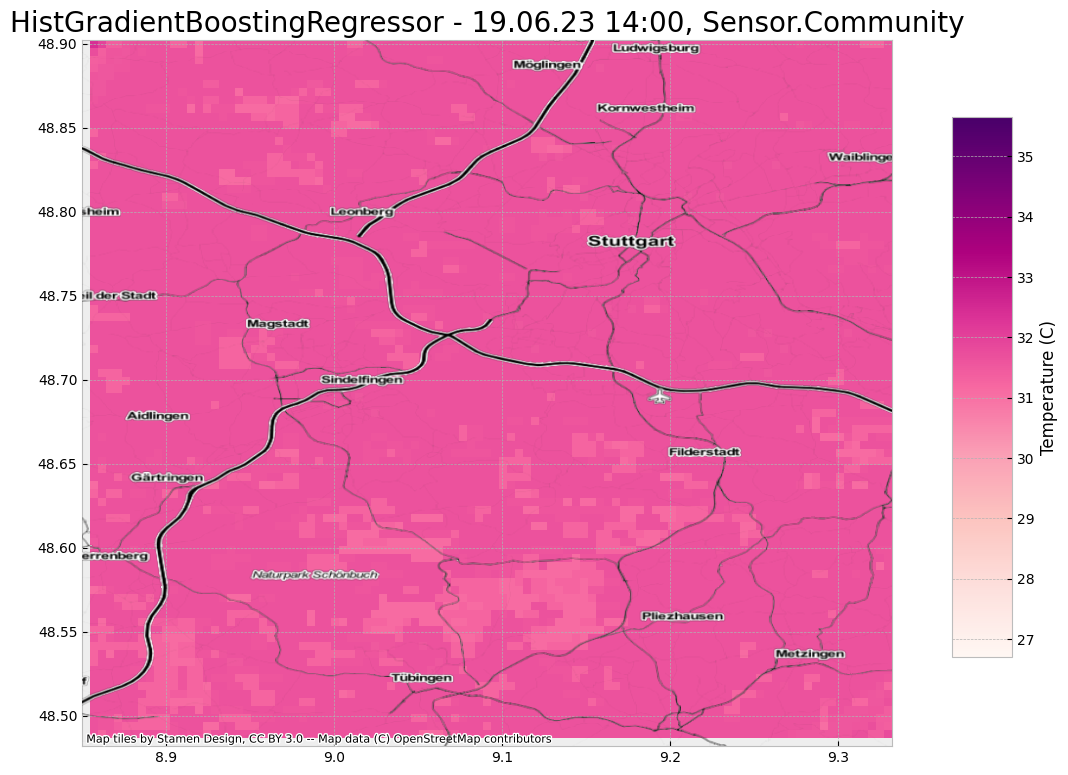
\includegraphics[width=0.9\textwidth]{images/eval areal interpolation hgb 14h.png}
    \caption{HistGradientBoostingRegressor Areal Interpolation, Sensor.Community Stuttgart, 19.06.2023 2PM}
    \label{fig:eval areal interpolation hgb 14h stuttgart}
\end{figure}

\subsection{Comparison with Kriging}

In order to evaluate the performance of the \gls{ml} model, we need to first get a better understanding of the interpolation quality of existing interpolation techniques. Next to simpler deterministic interpolation methods, such as \gls{idw} that are simple but performant, yet struggle to capture more complex interdependencies, there are also more complex methods available. The most common geostatistical method for interpolation is Kriging.\\
In the scope of this work, we unfortunately cannot compare available Kriging methods with each other and therefore need to focus on a subset of methods, namely those easily available via the pykrige Python library, i.e., Ordinary and Universal Kriging. We note however, that for example according to~\cite{njoku2023effects}, there are many other more sophisticated and specialised Kriging methods such as EBK and EBKRP that could perform better. For \gls{ok}, we use the same dataset we used previously but only use the coordinates and the target \gls{ta}. With a 80\% train and 20\% test split, we achieved the following \gls{rmse} and \gls{r2} scores in Table~\ref{tab: areal interpolation ok 2pm}. If we choose the same data and train and test our \gls{ml} models on it, we get the \gls{rmse} and \gls{r2} shown in Table~\ref{tab: areal interpolation ml models 2pm}.\\

\begin{table}[ht]
  \centering
  \begin{tabular}{lrr}
  \toprule
  Variogram Model &     \gls{rmse} &        \gls{r2} \\
  \midrule
          linear & 1.712089 & -0.001049 \\
            power & 1.712089 & -0.001049 \\
        gaussian & 1.327896 &  0.397814 \\
        spherical & 1.272819 &  0.446732 \\
      exponential & 1.471249 &  0.260778 \\
  \bottomrule
  \end{tabular}
  \label{tab: areal interpolation ok 2pm}
  \caption{\gls{rmse} and \gls{r2} of Ordinary Kriging for Stuttgart 19.06.2023 2PM, Sensor.Community}

  \begin{tabular}{lrr}
  \toprule
            ML Model &     \gls{rmse} &       \gls{r2} \\
  \midrule
            KNeighborsRegressor & 1.314883 & 0.183336 \\
          RandomForestRegressor & 1.205100 & 0.314014 \\
  HistGradientBoostingRegressor & 1.098671 & 0.429831 \\
                            SVR & 1.432225 & 0.031072 \\
  \bottomrule
  \end{tabular}
  \label{tab: areal interpolation ml models 2pm}
  \caption{\gls{rmse} and \gls{r2} of \gls{ml} Models for Stuttgart 19.06.2023 2PM, Sensor.Community}
\end{table}

From these results we can see, that our \gls{ml} models outperform \gls{ok} in terms of \gls{rmse} but lack behind in \gls{r2} score. To show the differences, we use both Kriging and \gls{hgb} to interpolate a map. The results of the best performing model according to \gls{r2} score, i.e., the spherical variogram, can be seen in Figure~\ref{fig:eval areal interpolation ok 14h stuttgart}. The \gls{hgb} results can be seen in Figure~\ref{fig:eval areal interpolation hgb 14h stuttgart}.\\

\begin{figure}[htp]
    \centering
    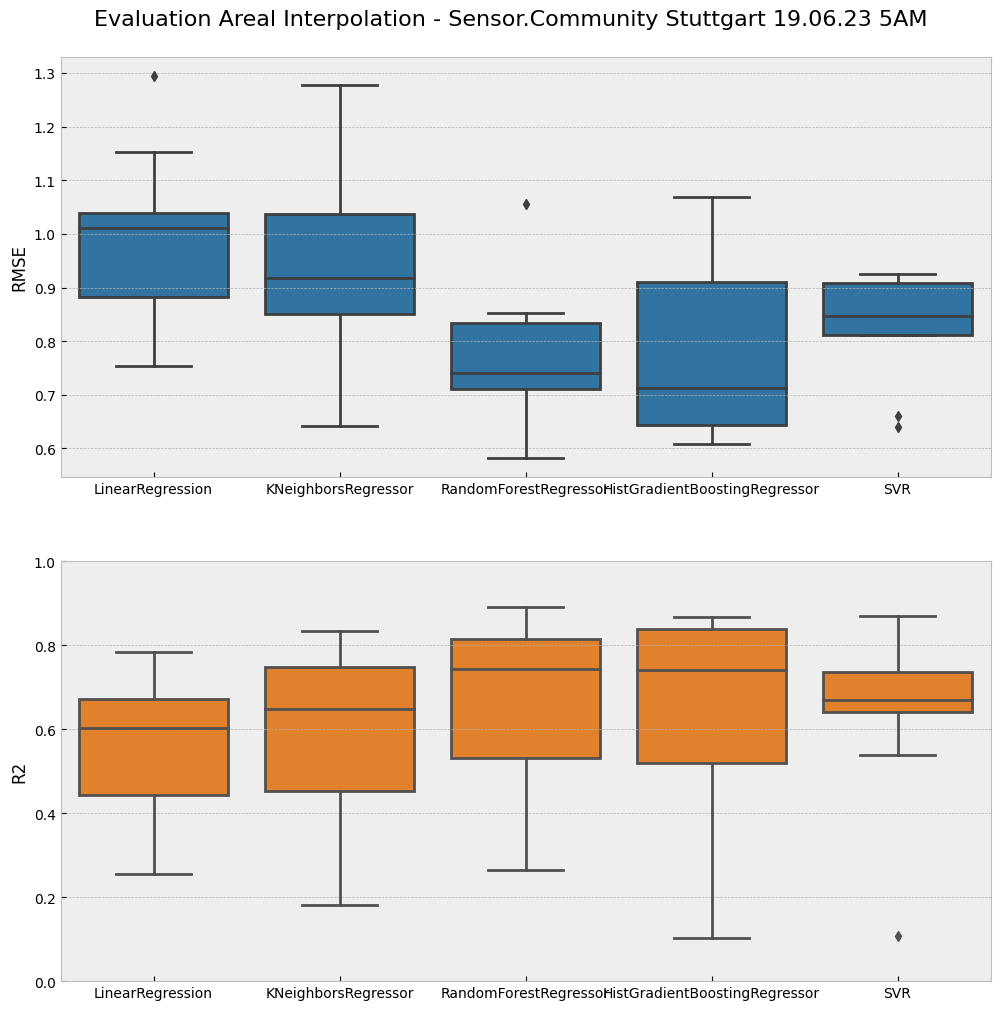
\includegraphics[width=0.8\textwidth]{images/eval areal interpolation 19.06.2023 5h.png}
    \caption{Areal Interpolation Comparison, Sensor.Community Stuttgart, 19.06.2023 5AM}
    \label{fig:eval areal interpolation 5h stuttgart}

    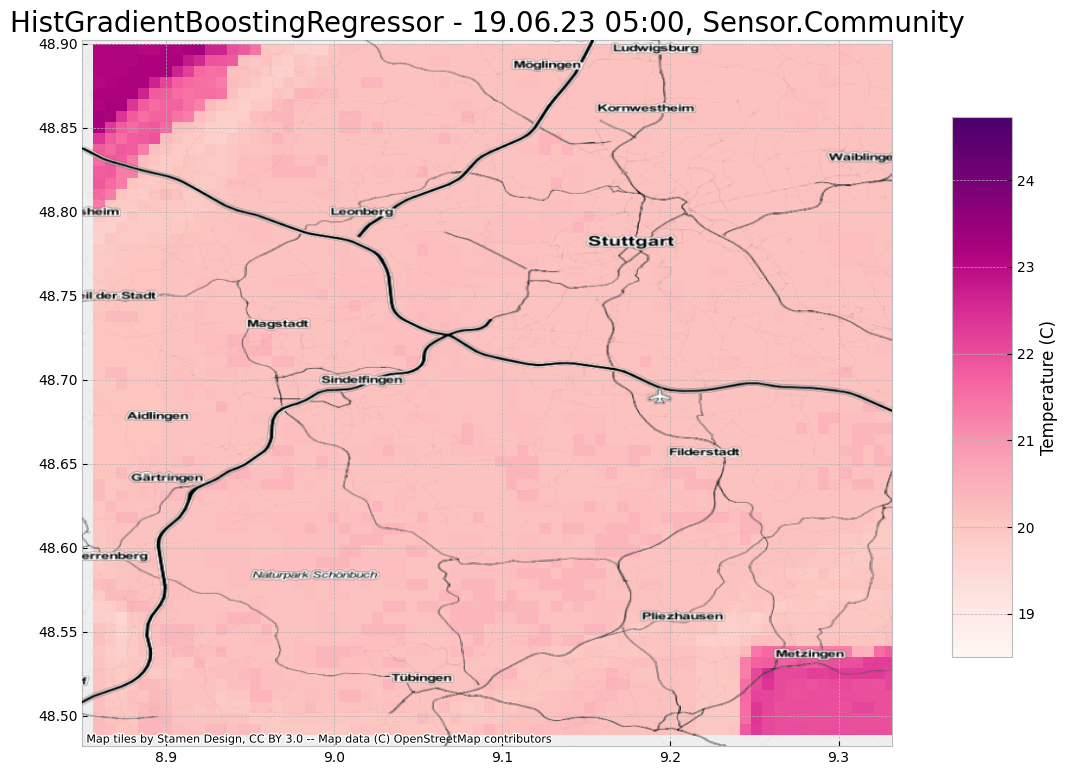
\includegraphics[width=0.8\textwidth]{images/eval areal interpolation hgb 5h.png}
    \caption{HistGradientBoostingRegressor Areal Interpolation, Sensor.Community Stuttgart, 19.06.2023 5AM}
    \label{fig:eval areal interpolation 5h stuttgart map}
\end{figure}

\subsection{Comparison during Night}

Next to mapping \gls{ta} when it's especially hot, we also take a look at night time \gls{ta} mapping to have a baseline for comparison and try to understand if there are differences. The results from the 10-fold cross validation on the same dataset but with the time set to 5am, i.e., the time of that day the \gls{ta} was lowest, can be found in Figure~\ref{fig:eval areal interpolation 5h stuttgart}. The \gls{hgb} model was then trained again with the error values in Table~\ref{tab: eval night time 5h stuttgart} and the resulting map in Figure~\ref{fig:eval areal interpolation 5h stuttgart map}.\\
We can clearly see, that \gls{r2} values during the night are way higher, suggesting that we miss some kind of information during the day, such as solar radiation and \gls{lst}, which might need to be integrated into our model for better prediction results. Additionally, we could also improve the accuracy by using Sentinel 2 and Landsat readings due to their way higher spatial resolution, as currently the \gls{modis} remote sensing values have a 500m pixel size in comparison to a pixel size of 10m to 50m. In that case however, we would also need to manually calculate \gls{ndvi} etc., which adds a little bit of extra work.

\begin{table}[ht]
  \centering
  \begin{tabular}{lrr}
  \toprule
                      ML Model &     \gls{rmse} &       \gls{r2} \\
  \midrule
            KNeighborsRegressor & 0.935147 & 0.679537 \\
          RandomForestRegressor & 0.730378 & 0.804515 \\
  HistGradientBoostingRegressor & 0.729455 & 0.805009 \\
                            SVR & 0.804774 & 0.762663 \\
  \bottomrule
  \end{tabular}
  \label{tab: eval night time 5h stuttgart}
\end{table}

\begin{figure}[ht]
    \centering
    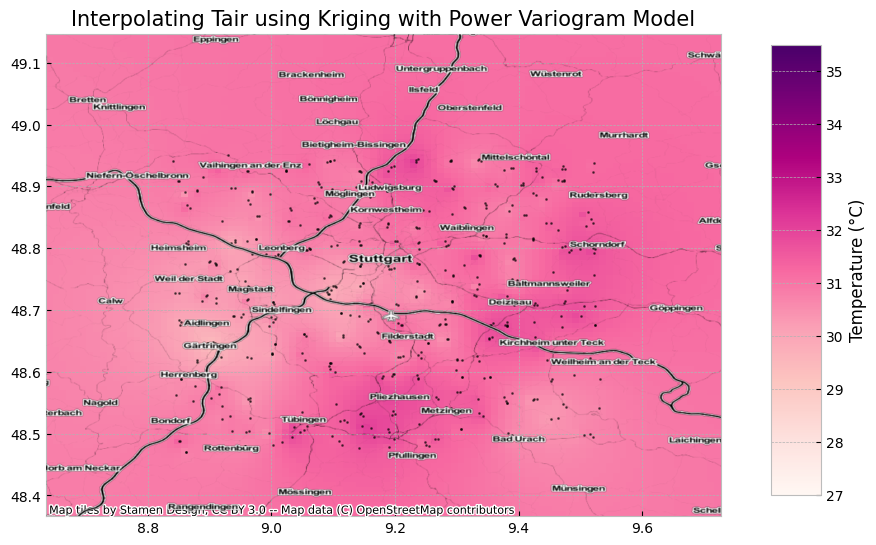
\includegraphics[width=0.9\textwidth]{images/eval areal interpolation ok stuttgart 14h netatmo.png}
    \caption{Ordinary Kriging Power Variogram, Netatmo Stuttgart, 19.06.2023 2PM}
    \label{fig:eval areal interpolation ok 14h stuttgart netatmo}
\end{figure}

\subsection{Comparison with Netatmo}

Like Sensor.Community, Netatmo also has many stations in the region of Stuttgart. To compare the two providers, we use Netatmo data for the same timestamp, i.e., 2PM on the 19. June 2023, to get a rough comparison. Please note, that we did not apply any \gls{qc} to this data. This comparison should be improved by also applying \gls{qc} steps to Netatmo stations; however, we did not have the time to collect this data and do the pre-processing steps in this work. The \gls{ok} results are shown in Table~\ref{tab: areal interpolation ok 2pm netatmo stuttgart}. In this comparison, the power variogram model seems to perform the best. The resulting map can be found in Figure~\ref{fig:eval areal interpolation ok 14h stuttgart netatmo}. The next step would be to also run through all pre-processing steps with Netatmo data for \gls{qc} etc.\ and also compare the \gls{ml} models with each other on the Netatmo data, possibly also on a combination of Netatmo and Sensor.Community to get even higher spatial coverage.

\begin{table}[ht]
  \centering
  \begin{tabular}{lrr}
  \toprule
  Variogram Model &     \gls{rmse} &       \gls{r2} \\
  \midrule
          linear & 1.755016 & 0.070271 \\
            power & 1.592532 & 0.234456 \\
        gaussian & 1.746884 & 0.078868 \\
        spherical & 1.722252 & 0.104662 \\
      exponential & 1.669650 & 0.158518 \\
  \bottomrule
  \end{tabular}
  \label{tab: areal interpolation ok 2pm netatmo stuttgart}
  \caption{\gls{rmse} and \gls{r2} of Ordinary Kriging for Stuttgart 19.06.2023 2PM, Netatmo}
\end{table}

% TODO: Optional add Hamburg
% \subsubsection{Hamburg}

% Todo: add Hamburg station locations\\

% TODO
% First compare only \gls{ta} for stations that are near a reference station and have enough buddies for sensor community
% - only for june 2023 from sensor community, not january as heat islands are not as important in winter (which depends on the context ofc if the goal is for example to save heating costs, could be a factor)

% Steps in the evaluation:
% - find sensor community stations near reference stations that passed m5 QC step
% - Compare different interpolation approaches
%   - linear, forests, KNN, NNetwork
%   - with different amounts of data available (99\% -> 1\%) and see how \gls{rmse} evolves


% Steps:
% - deterministic approaches
%   - "naive" approach with nearest neighbor -> show high error rate
% - probabilistic approaches
%   - reference approach with geostatistical methods (ordinary kriging, empirical bayesian kriging, EBK with regression) -> still high error rate, especially with lower density of weather stations/bad support for irregularly spaced data
%     - ordinary kriging:
%         - temperature semivariogram first
%         - add additional features (e.g., soil temperature, land coverage, sky view factor, ...) as semivariograms and use cokrigin to combine them
%     - empirical bayesian kriging:
%         - not implemented out of the box (pykrige)

%   - semivariogram: https://pro.arcgis.com/en/pro-app/latest/help/analysis/geostatistical-analyst/understanding-a-semivariogram-the-range-sill-and-nugget.htm

% - deep learning approach with neural networks -> iteratively improve model by adding additional features, compare with reference approach

% % Overall steps

% 1. Data Collection and rough analysis
%   1.1. Get data from Sensor.Community
%   1.2. Get data from DWD
%   1.3. Get data from satellites via Google Earth Engine
%   1.4. Get data from Netatmo (Hamburg, try to get Stuttgart as reference with historical data via API)
% 2. QC steps (TA first)
%   2.1. Try to remove indoor stations and stations with irregular data
%   2.2. Remove stations based on buddy check (removes a lot of sensor community stations due to lower density)
%   2.3. Reference station has high-quality data already, but can be used as a reference (interesting the comparison from 2m TA to 5cm TA)
%   2.4. Discuss QA for other parameters (Humidity, Pressure etc.)
% 3. Comparison of models
%   3.1. Simple models with only coordinates as input features and TA as target feature
%   3.2. Add additional features (land coverage (\gls{ndvi}, EVI)) and see how they improve the model
%     3.2.1. For land coverage etc.\ compare different satellites and resolutions
%     3.2.2. For coordinates/distances, compare different ways of calculating distances or modelling them in the model
%     3.2.3. Compare influence of normalization
%   3.3. Try to create a more complex NN model to show capabilities of NNs and try out LSTM for time series
%   3.4. Choose final candidate that seems the most promissing and compare with reference approach
% 4. Comparison with reference approaches
%   4.1. Compare with simple Ordinary Kriging approach (with different kernels)
%   4.2. Discuss problem of not being able to extrapolate